\documentclass[12pt,a4paper]{article}
\usepackage[utf8]{inputenc}
\usepackage[english]{babel}
%\usepackage{minted}
\usepackage{listings}
\usepackage{xcolor}
\usepackage{graphicx}

%For syntax highlighting
\definecolor{codegreen}{rgb}{0,0.6,0}
\definecolor{codegray}{rgb}{0.5,0.5,0.5}
\definecolor{codepurple}{rgb}{0.58,0,0.82}
\definecolor{backcolour}{rgb}{1,1,1}

%%Sets different parameters
\lstdefinestyle{mystyle}{
	backgroundcolor=\color{backcolour},   
    commentstyle=\color{codegreen},
    keywordstyle=\color{magenta},
    numberstyle=\tiny\color{codegray},
    stringstyle=\color{codepurple},
    basicstyle=\ttfamily\footnotesize,
    breakatwhitespace=false,         
    breaklines=true,                 
    captionpos=b,                    
    keepspaces=true,                 
    numbers=left,                    
    numbersep=5pt,                  
    showspaces=false,                
    showstringspaces=false,
    showtabs=false,                  
    tabsize=4
}
\lstset{style=mystyle}

\title{\bf Code Conversion}
\author{\vspace{-10ex}}
\date{\vspace{-10ex}}
\begin{document}
\maketitle

\begin{minipage}{0.45\textwidth}
        \begin{tabular}{l l}
            \textbf{Expt No:}&4\\
            \textbf{Date :}&18/09/2020
        \end{tabular}
\end{minipage}%
\begin{minipage}{0.45\textwidth}
        \begin{tabular}{l l}
             \textbf{Name:}& Shivanirudh S G  \\
             \textbf{Reg No:} & 185001146 
        \end{tabular}
\end{minipage}
\vspace{1cm}
\hrule

\begin{flushleft}
\subsection*{\textbf{Aim:}} 
To perform code conversion in 8086.

\vspace{1cm}
\hrule
\subsection*{\textbf{\underline{BCD to Hexadecimal}}}

\subsubsection*{\textbf{Algorithm:}}
\begin{itemize}
    \item Move the data segment to the AX register and then move it to the DS register.
    \item Move hexadecimal value 0A to DL register, 04 to CL register, and 00 to BH register.
    \item Move BCD value to AL register.
    \item Perform AND operation with AND AL, F0H to mask the lower byte. 
    \item Shift AL register 4 bits to right by SHR AL, CL.
    \item Multiply AL with DL register with MUL DL.
    \item Move BCD value to BL register.
    \item Perform AND operation with AND BL, 0FH to mask the upper byte.
    \item Add value in BX register to AX register using ADD AX, BX.
    \item Store result in HEX from AX register.
\end{itemize}

\newpage
\subsubsection*{\textbf{Program:}}

\begin{table}[htb]
\centering
\resizebox{\columnwidth}{!}{
\begin{tabular}{|l|l|} 
\hline
\textbf{Program}                                                 & \textbf{Comments}                             \\ 
\hline
\hline
assume cs:code, ds:data                                          & Declare code and data segments                \\
\hline
data segment                                                     & Start of data segment                         \\
\hline 
bcd db 34H                                                       & Define byte bcd with value 34                 \\
\hline
hex dw 0000H                                                     & Define word hex with hex value 0000           \\
\hline
data ends                                                        & End of data segment                           \\
\hline
code segment                                                     & Start of code segment                         \\
\hline
start:~mov ax, data                                              & Move data to AX register                      \\
\hline
mov ds, ax                                                       & Move contents of AX register to DS register   \\
\hline
mov dl, 0AH                                                      & Move hex value 0A to DL register              \\
\hline
mov al, bcd                                                      & Move contents of bcd to AL register           \\
\hline
and al, 0F0H                                                     & Perform AL = Al \& F0                         \\
\hline
mov cl, 04H                                                      & Move hex value 04 to CL register              \\
\hline
shr al, cl                                                       & Shift AL register right by 04 bits            \\
\hline
mul dl                                                           & Perform AX = AL x DL                          \\
\hline
mov bl, bcd                                                      & Move contents of bcd to BL register           \\
\hline
and bl, 0F0H                                                     & Perform BL = Bl \& 0F                         \\
\hline
mov bh, 00H                                                      & Move hex value 00 to CL register              \\
\hline
add ax, bx                                                       & Perform AX = AX + BX                          \\
\hline
mov hex, ax                                                      & Move contents of AX register to HEX           \\
\hline
int 21h                                                          & Request interrupt routine                     \\ 
\hline
code ends                                                        & End of code segment                           \\
\hline
end start                                                        &                                               \\
\hline
\end{tabular}
}
\end{table}

\newpage
\subsection*{\textbf{Unassembled code:}}
\begin{figure}[h]
    \centering
    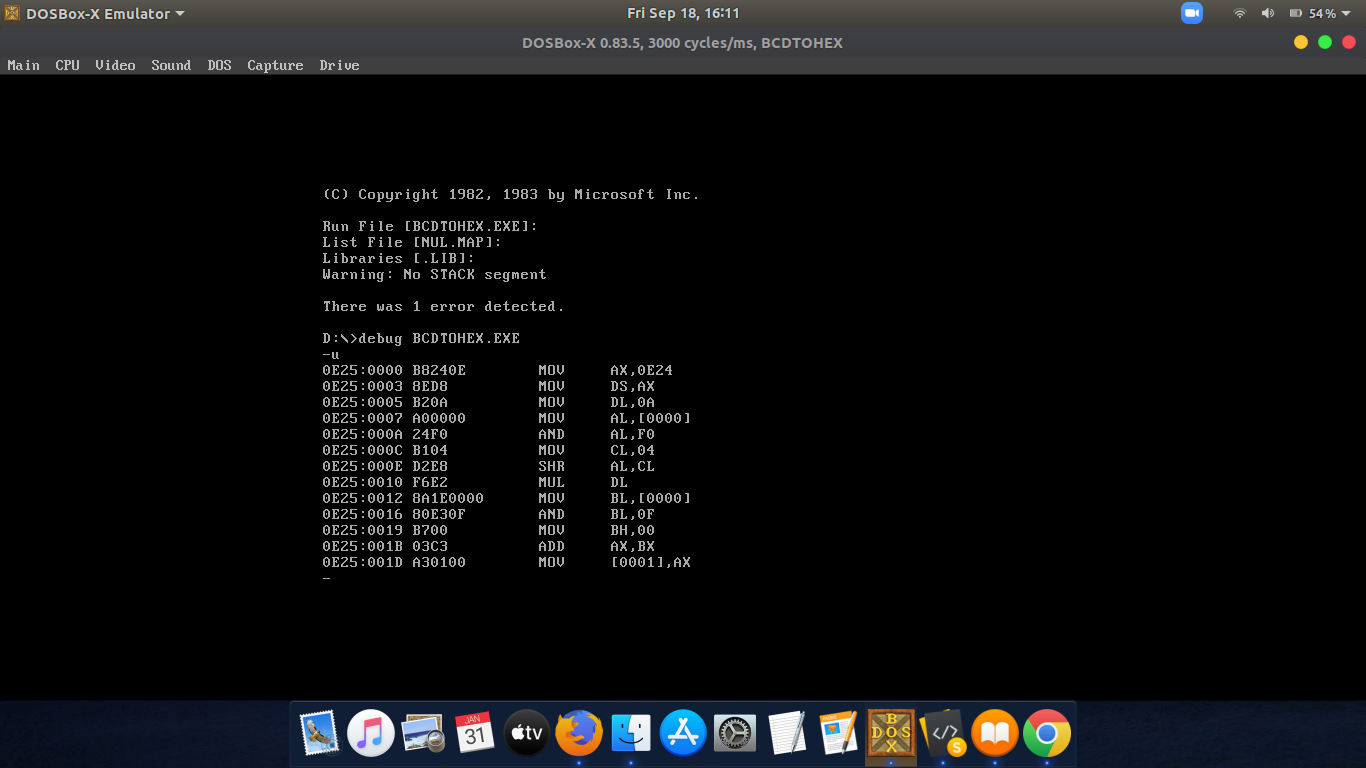
\includegraphics[trim = 100mm 60mm 200mm 120mm, clip, width = \textwidth]{Pics/BHUS.png}
\end{figure}
\subsubsection*{\textbf{Input and Output:}}
\begin{figure}[h]
    \centering
    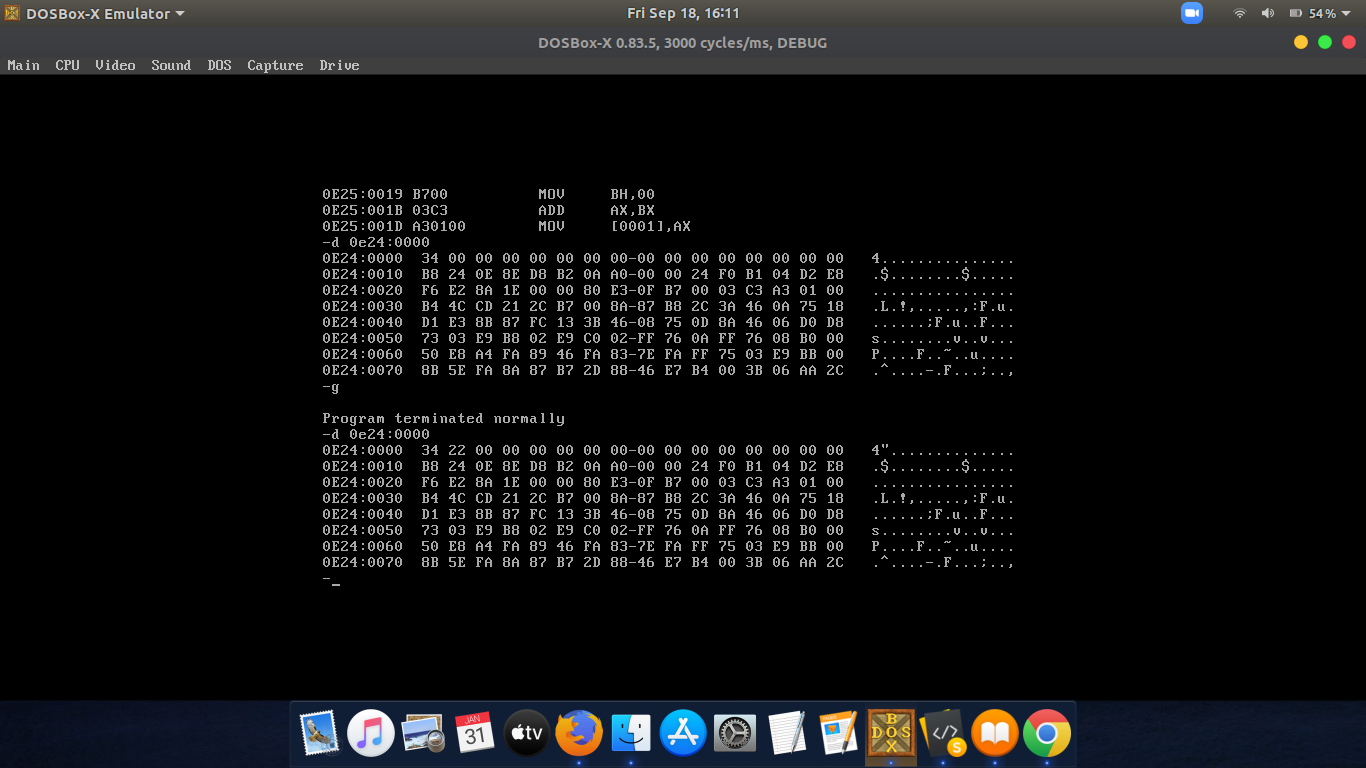
\includegraphics[trim = 100mm 60mm 100mm 80mm, clip, width = \textwidth]{Pics/BHIO.png}
    \caption{ \textbf{Input:} \emph{BCD:} 34 ; \newline \hspace{1cm}
              \textbf{Output:} \emph{Hexadecimal:} 22H}
\end{figure}
%-------------------------------------------------------------------------------------------------------------------------------------------
\newpage
\subsection*{\textbf{\underline{Hexadecimal to BCD}}}

\subsubsection*{\textbf{Algorithm:}}
\begin{itemize}
    \item Move the data segment to the AX register and then move it to the DS register.
    \item Move hexadecimal value 0A to CH register, and 64 to CL register.
    \item Move HEX value to AL register, 00H to AH register.
    \item Divide AX by Cl using DIV CL.
    \item Store quotient from AL in BCDU.
    \item Move value of AH to AL register, and 00H to AH register. 
    \item Divide AX by CH using DIV CH.
    \item Move 04H to the CL register.
    \item Move value of AH register to CH register.
    \item Shift AL register 4 bits to left by SHL AL, CL.
    \item Add CH to AL register using ADD AL, CH.
    \item Move contents of AL register to BCDL.
\end{itemize}

\newpage
\subsubsection*{\textbf{Program:}}

\begin{table}[htb]
\centering
\resizebox{\columnwidth}{!}{
\begin{tabular}{|l|l|} 
\hline
\textbf{Program}                                                 & \textbf{Comments}                             \\ 
\hline
\hline
assume cs:code, ds:data                                          & Declare code and data segments                \\
\hline
data segment                                                     & Start of data segment                         \\
\hline 
bcd_u db 00H                                                     & Define byte bcd_u with value 00               \\
\hline
bcd_l db 00H                                                     & Define byte bcd_l with value 00               \\
\hline
hex dw 0FDH                                                      & Define byte hex with hex value FD             \\
\hline
data ends                                                        & End of data segment                           \\
\hline
code segment                                                     & Start of code segment                         \\
\hline
start:~mov ax, data                                              & Move data to AX register                      \\
\hline
mov ds, ax                                                       & Move contents of AX register to DS register   \\
\hline
mov cl, 64H                                                      & Move hex value 64 to CL register              \\
\hline
mov ch, 0AH                                                      & Move hex value 0A to CH register              \\
\hline
mov al, hex                                                      & Move contents of bcd to AL register           \\
\hline
mov ah, 00H                                                      & Move hex value 00 to AH register              \\
\hline
div cl                                                           & Perform AL = AX / CL                          \\
\hline         
mov bcdu, al                                                     & Move contents of AL register to bcdu          \\
\hline
mov al, ah                                                       & Move contents of AH register to AL            \\
\hline
mov ah, 00H                                                      & Move hex value 00 to AH register              \\
\hline
div ch                                                           & Perform AL = AX / CH                          \\
\hline
mov cl, 04H                                                      & Move hex value 04 to CL register              \\
\hline
mov ch, ah                                                       & Move contents of AH to CH register            \\
\hline
shl al, cl                                                       & Shift AL register left by 04 bits             \\
\hline
add al, ch                                                       & Perform AL = AL + CH                          \\
\hline
mov bcdl, al                                                     & Move contents of AL to bcdl register          \\
\hline
int 21h                                                          & Request interrupt routine                     \\ 
\hline
code ends                                                        & End of code segment                           \\
\hline
end start                                                        &                                               \\
\hline
\end{tabular}
}
\end{table}

\newpage
\subsection*{\textbf{Unassembled code:}}
\begin{figure}[h]
    \centering
    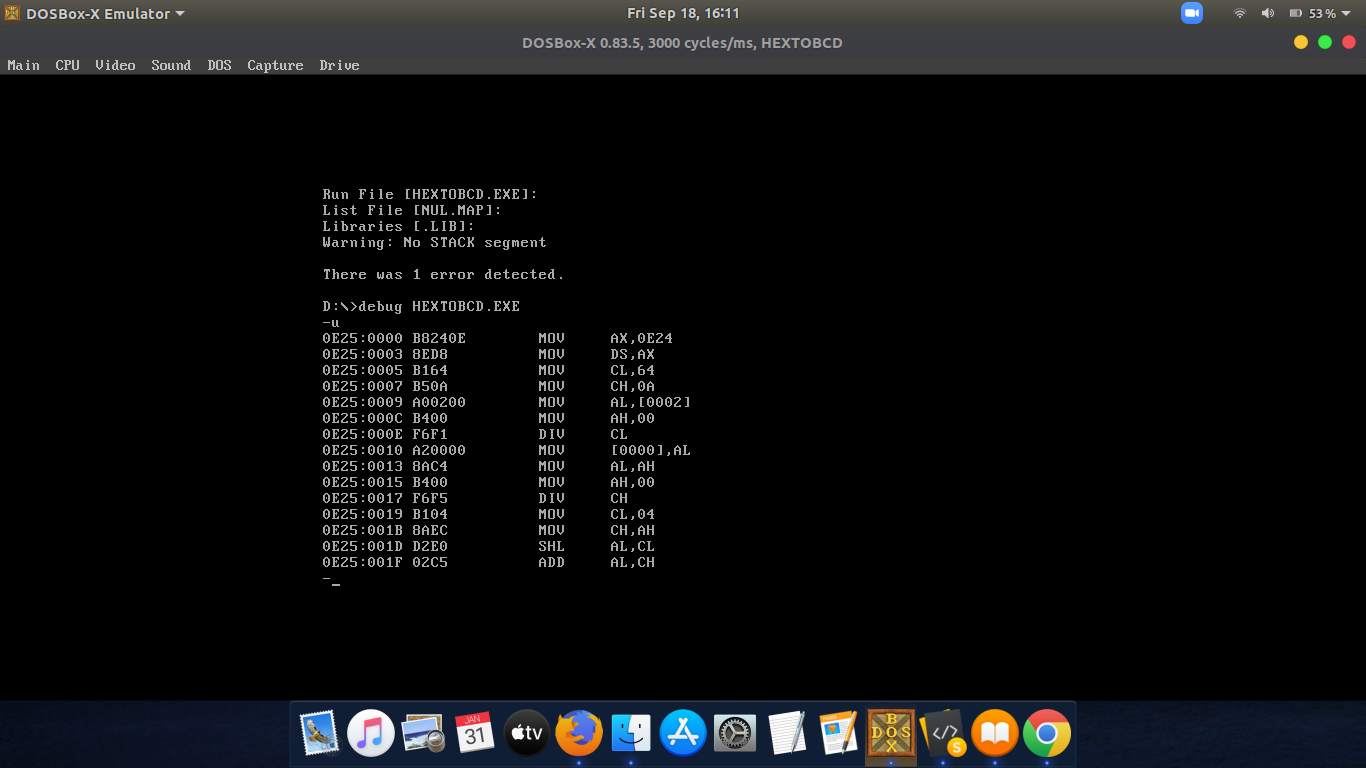
\includegraphics[trim = 100mm 60mm 200mm 110mm, clip, width = \textwidth]{Pics/HBUS.png}
\end{figure}
\subsubsection*{\textbf{Input and Output:}}
\begin{figure}[h]
    \centering
    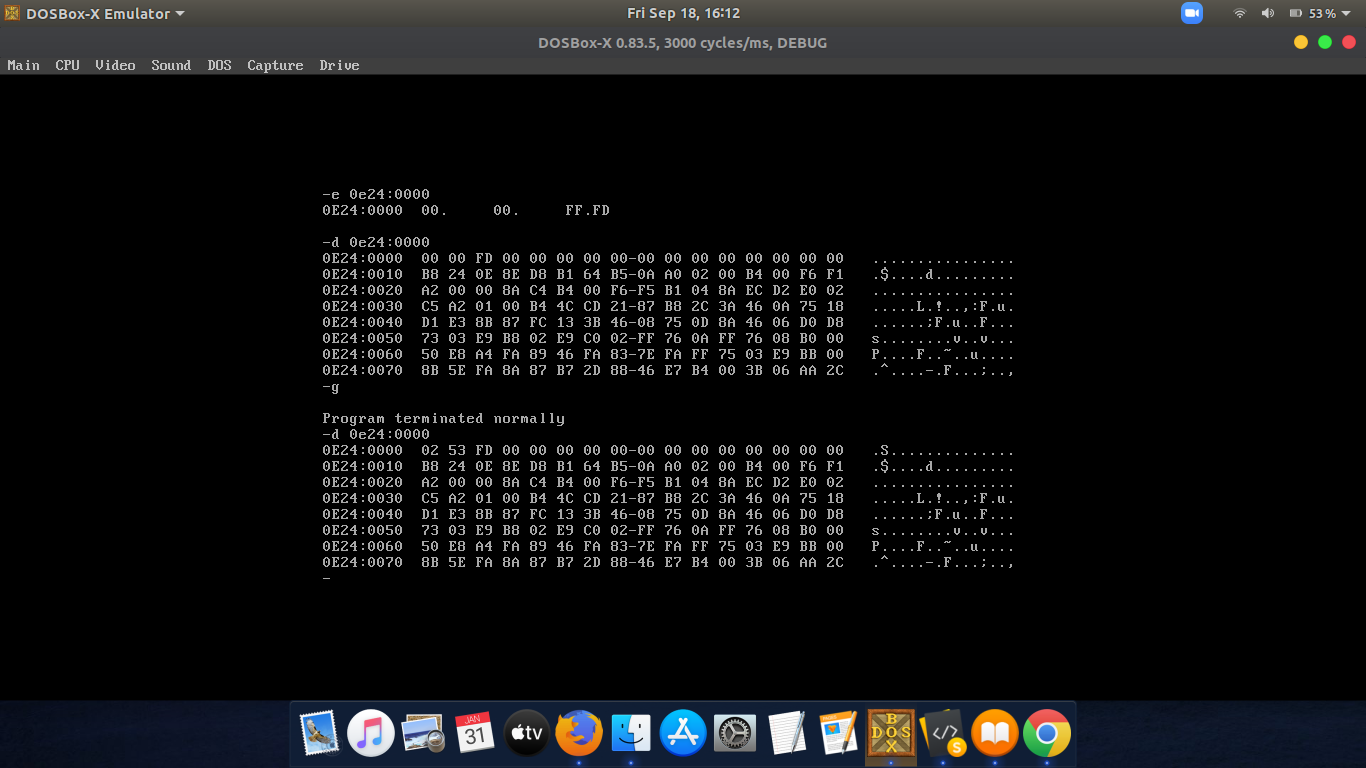
\includegraphics[trim = 100mm 60mm 100mm 80mm, clip, width = \textwidth]{Pics/HBIO.png}
    \caption{ \textbf{Input:} \emph{Hexadecimal:} FDH ; \newline \hspace{1cm}
              \textbf{Output:} \emph{BCD:} 253}
\end{figure}
\hrule
\subsection*{\textbf{Result:}}
The 8086 programs were written to perform code conversion from BCD to Hexadecimal and vice versa, and the results observed.
\end{flushleft}
\end{document}